% Kapitel 5: Demonstration und Evaluation

\chapter{Demonstration und Evaluation}
\label{chap:demonstration}

Dieses Kapitel prüft das entwickelte Artefakt anhand einer szenariobasierten Demonstration (Abschnitt~\ref{sec:demonstration-szenarien}), dokumentiert das Evaluationsdesign (Abschnitt~\ref{sec:evaluationsdesign}), stellt die Ergebnisse dar (Abschnitt~\ref{sec:evaluationsergebnisse}) und reflektiert den Prozess (Abschnitt~\ref{sec:reflexion}).

\section{Szenariobasierte Demonstration}
\label{sec:demonstration-szenarien}

Die Demonstration erfolgt anhand zweier fiktiver Szenarien, die vom Autor konstruiert und bewertet wurden. Die Ergebnisse illustrieren die Bewertungsmechanik; sie sind keine empirisch validierten Befunde. Da der Autor die Indikatoren selbst entwickelt hat, ist ein \textit{Confirmation Bias} nicht auszuschließen: Die Bewertung könnte unbewusst auf die gewünschten Differenzierungsmuster hin erfolgt sein.

Die Szenarien weisen nach Peffers et al. die \textit{Utility} des Artefakts nach \autocite{Peffers2007}. Im FEDS-Framework ordnet sich die szenariobasierte Demonstration als \textit{künstliche Evaluation} ein \autocite{Venable2016}. Die Szenarien variieren in Hochrisiko-Kategorie (Anhang~III), Organisationsgröße und Governance-Ausgangsniveau (Abschnitt~\ref{sec:evaluationsmethode}).

\textbf{Szenario~1 -- Kreditscoring (Finanzsektor):} Hochrisiko gemäß Anhang~III Nr.~5(b) (Kreditwürdigkeitsprüfung); mittleres Finanzinstitut (500--1.000~Mitarbeitende) mit MaRisk-Compliance-Strukturen und zertifiziertem ISMS nach ISO~27001. Das KI-System ist ein Gradient-Boosting-Ensemble-Modell in der bestehenden Kreditvergabe-Pipeline. \textbf{Stärken:} D1~Risikomanagement~(3,2) -- die BaFin-MaRisk-Anforderungen haben ein auf KI übertragbares Risikomanagementsystem geschaffen; D6~Technische Robustheit~(3,4) -- IT-Sicherheitsstandards und Penetrationstests sind etabliert; D5~Menschliche Aufsicht~(3,0) -- das Vier-Augen-Prinzip bei Kreditentscheidungen ist regulatorisch verankert. \textbf{Schwächen:} D4~Transparenz~(2,0) -- XAI-Methoden (SHAP, LIME) werden punktuell eingesetzt, aber nicht in standardisierte Erklärungsprozesse überführt; die Art.~13-Informationspflichten gegenüber Kreditnehmern sind nicht formalisiert; D2~Data Governance~(2,4) -- Datenqualitätsprozesse fokussieren auf regulatorische Meldepflichten, systematisches Bias-Monitoring für geschützte Merkmale fehlt. \textbf{Gesamtscore: 2,77} (Defined, unteres Niveau); die Gap-Analyse identifiziert D4 als kritisch (Gap:~1,0) und D2 als moderat (Gap:~0,6). Die KI-gestützte Tiefenanalyse empfiehlt kurzfristig ein XAI-Standardverfahren für Kreditentscheidungserklärungen, mittelfristig eine Bias-Monitoring-Pipeline mit Protected-Attribute-Analyse.

\textbf{Szenario~2 -- KI-gestütztes Recruiting (Technologiesektor):} Hochrisiko gemäß Anhang~III Nr.~4(a) (Beschäftigungsverhältnisse); Scale-up (200~Mitarbeitende) mit intern entwickeltem NLP-Modell zur Lebenslauf-Vorauswahl im Pilotbetrieb. \textbf{Stärken:} D5~(3,2) -- HR-Prozesse sehen manuelle Prüfung aller KI-Vorauswahlen vor; D3~(2,6) -- grundlegende Modelldokumentation vorhanden. \textbf{Schwächen:} D2~(1,8) -- kein systematisches Bias-Monitoring; geschlechtsspezifische und altersbezogene Verzerrungen, die bei NLP-Rekrutierungssystemen dokumentiert sind \autocite{Holtz2025}, werden nicht geprüft; D6~(2,0) -- keine Drift-Erkennung, keine definierten Genauigkeitsmetriken. \textbf{Gesamtscore: 2,38} (Managed); D2 und D6 sind kritisch (Gaps:~1,2 bzw.~1,0).

Die Prototyp-Oberfläche ist in Anhang~\ref{app:prototyp} dokumentiert. Das Dashboard (Abb.~\ref{fig:screenshot-dashboard}) zeigt die sechs Dimensionen mit Artikelzuordnung, das Scoping-Formular (Abb.~\ref{fig:screenshot-scoping}) ordnet das KI-System kontextuell ein, und die Assessment-Oberfläche (Abb.~\ref{fig:screenshot-assessment}) zeigt die Kriterienbewertung mit aufklappbaren Reifegrad-Indikatoren (Abb.~\ref{fig:screenshot-indikatoren}). Die Ergebnisseite umfasst Radar-Chart (Abb.~\ref{fig:screenshot-radar}), Gap-Analyse (Abb.~\ref{fig:screenshot-gap}), Compliance-Heatmap (Abb.~\ref{fig:screenshot-heatmap}) und Maßnahmenpläne (Abb.~\ref{fig:screenshot-aktionsplan}).

\textbf{Exemplarischer Bewertungsprozess -- D2 in Szenario~2:} Die folgende Tabelle zeigt die Bewertung von D2~(Data Governance) in Szenario~2 kriterienweise. Die bewertende Person ordnet den Ist-Zustand jeweils einer Reifegradstufe zu (vollständige Indikatoren in Anhang~\ref{app:bewertungsdimensionen}):

\begin{table}[htbp]
\centering
\caption{Exemplarische Kriterienbewertung: D2 Data Governance in Szenario~2 (Recruiting)}
\label{tab:walkthrough-d2}
\small
\renewcommand{\arraystretch}{1.2}
\begin{tabular}{|l|c|p{7.5cm}|}
\hline
\textbf{Kriterium} & \textbf{Score} & \textbf{Begründung der Stufenzuordnung} \\
\hline
D2.1 Datenqualitätsstandards & 2 & Grundlegende Qualitätsprüfungen für Lebenslaufdaten existieren (Vollständigkeitschecks), sind jedoch nicht in dokumentierten Standards formalisiert. Stufe~2 (Managed): ``Grundlegende Maßnahmen etabliert, nicht standardisiert.'' \\
\hline
D2.2 Bias-Erkennung & 1 & Keine systematische Analyse geschützter Merkmale in den Trainingsdaten. Weder geschlechtsspezifische noch altersbezogene Verzerrungen werden geprüft \autocite{Holtz2025}. Stufe~1 (Initial): ``Bias wird nicht systematisch adressiert.'' \\
\hline
D2.3 Data Lineage & 2 & Trainingsdaten-Herkunft ist informell bekannt (interne Bewerberdatenbank), jedoch nicht systematisch dokumentiert. Stufe~2: ``Datenherkunft teilweise nachvollziehbar.'' \\
\hline
D2.4 DSGVO-Integration & 2 & DSGVO-Grundanforderungen (Einwilligung, Löschfristen) werden im HR-Prozess erfüllt; eine Integration mit KI-spezifischen Anforderungen (Art.~10 Abs.~5 zur Verarbeitung sensibler Daten für Bias-Erkennung) fehlt. Stufe~2. \\
\hline
D2.5 Kont. Datenqualität & 2 & Einmalige Datenaufbereitung vor dem Training; kein periodisches Re-Assessment der Datenqualität oder Monitoring auf Verteilungsverschiebungen. Stufe~2: ``Punktuelle Prüfung.'' \\
\hline
\multicolumn{2}{|r|}{\textbf{DimScore\textsubscript{D2}}} & $\frac{2+1+2+2+2}{5} = \mathbf{1{,}8}$ \\
\hline
\end{tabular}
\end{table}

Die Bewertung illustriert drei Eigenschaften des Assessment-Prozesses: Erstens stützt sich die Stufenzuordnung auf den Abgleich mit den Reifegrad-Indikatoren -- nicht auf subjektive Globaleinschätzung. Zweitens zeigt D2.2~(Bias-Erkennung, Score~1) als Ausreißer, dass ein einzelnes Kriterium auf Stufe~1 den Dimensionsdurchschnitt senkt und prioritären Handlungsbedarf signalisiert. Drittens wird die Gap-Berechnung nach Gleichung~\ref{eq:gap} nachvollziehbar: $\text{Gap}_{\text{D2}} = \max(0, \; 3{,}0 - 1{,}8) = 1{,}2$ -- ein signifikanter Gap ($1{,}0 \leq \text{Gap} < 2{,}0$). Die KI-gestützte Tiefenanalyse empfiehlt daher als kurzfristige Maßnahme eine Protected-Attribute-Analyse für das NLP-Modell.

Wie eingangs dargelegt, demonstrieren die Szenarien die \textit{funktionale} Differenzierungsfähigkeit des Frameworks (unterschiedliche Profile, Gaps, Empfehlungen), nicht dessen \textit{externe} Validität. Eine unabhängige Bewertung derselben Szenarien durch zwei der acht Evaluierenden hätte die Interrater-Reliabilität prüfen können, wurde aber aus Zeitgründen nicht realisiert.

\textbf{Szenarienvergleich und Differenzierungsfähigkeit:} Unter dieser Einschränkung zeigt der Vergleich die Differenzierungsfähigkeit auf vier Ebenen: (1)~\textit{Branchenspezifische Profile} -- der Finanzsektor profitiert von bestehenden regulatorischen Strukturen (MaRisk, ISMS), was höhere Scores bei D1 und D6 ergibt; das Scale-up zeigt Stärken bei D5, da HR-Prozesse als Kontrollinstanz wirken. (2)~\textit{Kontextabhängige Priorisierung} -- D2 ist in beiden Szenarien defizitär, aber mit unterschiedlichem Schweregrad (Gap~0,6 vs.~1,2). (3)~\textit{Differenzierte Handlungsempfehlungen} -- im Finanzsektor empfiehlt das Framework die Integration in MaRisk-Prozesse, im Scale-up den Aufbau grundlegender Governance-Strukturen. (4)~\textit{Scoring-Sensitivität} -- die Gesamtscores (2,38--2,77) bilden graduelle Unterschiede ab, ohne extreme Ausschläge zu produzieren.


\subsection{Radar-Chart-Vergleich der Szenarien}
\label{subsec:radar-overlay}

Die in den vorangegangenen Abschnitten tabellarisch dargestellten Dimensionsscores lassen sich als Radar-Chart überlagern, um die Governance-Profile auf einen Blick vergleichbar zu machen. Abbildung~\ref{fig:radar-overlay} zeigt die sechs Dimensionen beider Szenarien sowie die Compliance-Baseline ($\theta = 3{,}0$) als Referenzlinie.

\begin{figure}[htbp]
\centering
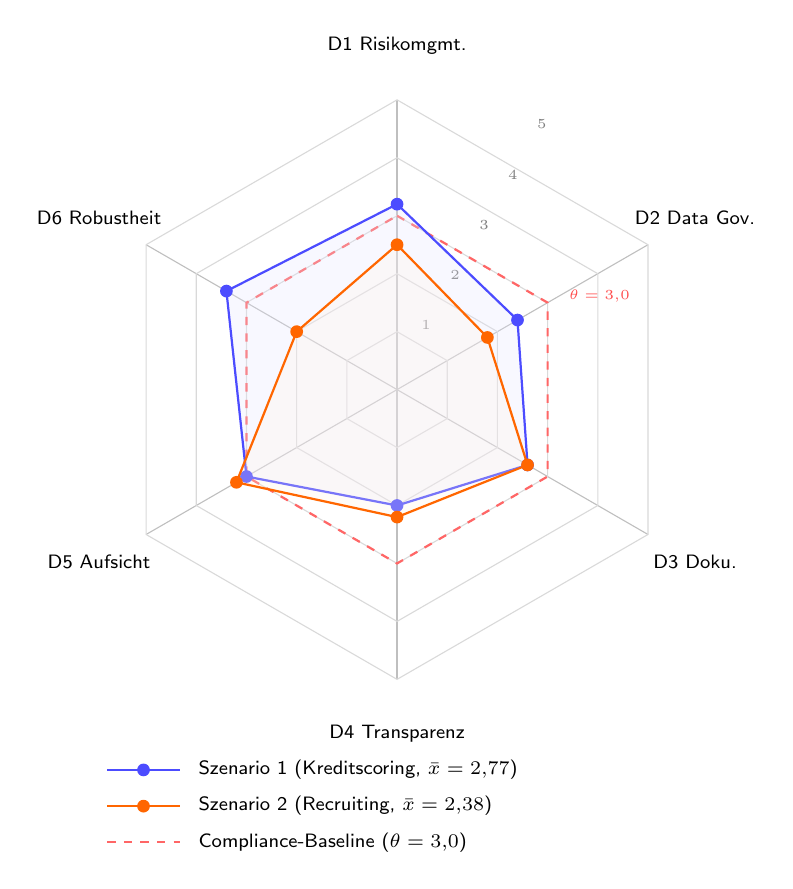
\begin{tikzpicture}[scale=1.15]
  % Definitionen
  \def\maxval{5}
  \def\levels{5}
  % Achsenwinkel (6 Dimensionen, Start oben, im Uhrzeigersinn)
  \foreach \i/\lab in {1/D1 Risiko\-mgmt., 2/D2 Data Gov., 3/D3 Doku., 4/D4 Transparenz, 5/D5 Aufsicht, 6/D6 Robustheit} {
    \pgfmathsetmacro{\angle}{90 - (\i-1)*60}
    % Gitterlinien
    \foreach \lev in {1,...,\levels} {
      \pgfmathsetmacro{\r}{\lev/\maxval*3.2}
    }
    % Achsen
    \draw[gray!50] (0,0) -- (\angle:3.2);
    % Labels
    \node[font=\sffamily\scriptsize, align=center] at (\angle:3.8) {\lab};
  }
  % Gitterpolygone
  \foreach \lev in {1,...,\levels} {
    \pgfmathsetmacro{\r}{\lev/\maxval*3.2}
    \draw[gray!30, thin]
      (90:\r) -- (30:\r) -- (-30:\r) -- (-90:\r) -- (-150:\r) -- (-210:\r) -- cycle;
    \node[font=\tiny, gray, anchor=south] at (60:\r) {\lev};
  }
  % Compliance-Baseline (theta = 3.0)
  \pgfmathsetmacro{\rbase}{3.0/\maxval*3.2}
  \draw[red!60, thick, dashed]
    (90:\rbase) -- (30:\rbase) -- (-30:\rbase) -- (-90:\rbase) -- (-150:\rbase) -- (-210:\rbase) -- cycle;
  \node[font=\sffamily\tiny, red!70, anchor=west] at (30:\rbase+0.15) {$\theta = 3{,}0$};
  % Szenario 1 – Kreditscoring (D1:3.2, D2:2.4, D3:2.6, D4:2.0, D5:3.0, D6:3.4)
  \pgfmathsetmacro{\ra}{3.2/\maxval*3.2}
  \pgfmathsetmacro{\rb}{2.4/\maxval*3.2}
  \pgfmathsetmacro{\rc}{2.6/\maxval*3.2}
  \pgfmathsetmacro{\rd}{2.0/\maxval*3.2}
  \pgfmathsetmacro{\re}{3.0/\maxval*3.2}
  \pgfmathsetmacro{\rf}{3.4/\maxval*3.2}
  \draw[blue!70, thick, fill=blue!10, fill opacity=0.25]
    (90:\ra) -- (30:\rb) -- (-30:\rc) -- (-90:\rd) -- (-150:\re) -- (-210:\rf) -- cycle;
  \foreach \val/\ang in {\ra/90, \rb/30, \rc/-30, \rd/-90, \re/-150, \rf/-210} {
    \fill[blue!70] (\ang:\val) circle (2pt);
  }
  % Szenario 2 – Recruiting (D1:2.5, D2:1.8, D3:2.6, D4:2.2, D5:3.2, D6:2.0)
  \pgfmathsetmacro{\ga}{2.5/\maxval*3.2}
  \pgfmathsetmacro{\gb}{1.8/\maxval*3.2}
  \pgfmathsetmacro{\gc}{2.6/\maxval*3.2}
  \pgfmathsetmacro{\gd}{2.2/\maxval*3.2}
  \pgfmathsetmacro{\ge}{3.2/\maxval*3.2}
  \pgfmathsetmacro{\gf}{2.0/\maxval*3.2}
  \draw[orange!80!red, thick, fill=orange!10, fill opacity=0.25]
    (90:\ga) -- (30:\gb) -- (-30:\gc) -- (-90:\gd) -- (-150:\ge) -- (-210:\gf) -- cycle;
  \foreach \val/\ang in {\ga/90, \gb/30, \gc/-30, \gd/-90, \ge/-150, \gf/-210} {
    \fill[orange!80!red] (\ang:\val) circle (2pt);
  }
  % Legende (zentriert unter dem Chart)
  \draw[blue!70, thick] (-3.2,-4.2) -- (-2.4,-4.2);
  \fill[blue!70] (-2.8,-4.2) circle (2pt);
  \node[font=\sffamily\scriptsize, anchor=west] at (-2.3,-4.2) {Szenario~1 (Kreditscoring, $\bar{x} = 2{,}77$)};
  \draw[orange!80!red, thick] (-3.2,-4.6) -- (-2.4,-4.6);
  \fill[orange!80!red] (-2.8,-4.6) circle (2pt);
  \node[font=\sffamily\scriptsize, anchor=west] at (-2.3,-4.6) {Szenario~2 (Recruiting, $\bar{x} = 2{,}38$)};
  \draw[red!60, thick, dashed] (-3.2,-5.0) -- (-2.4,-5.0);
  \node[font=\sffamily\scriptsize, anchor=west] at (-2.3,-5.0) {Compliance-Baseline ($\theta = 3{,}0$)};
\end{tikzpicture}
\caption{Radar-Chart-Overlay: Governance-Profile beider Szenarien mit Compliance-Baseline}
\label{fig:radar-overlay}
\end{figure}

Die Visualisierung macht Zusammenhänge sichtbar, die in der tabellarischen Darstellung verborgen bleiben.

Erstens zeigen die \textit{komplementären Stärke-Schwäche-Profile} ein Spiegelbild: Szenario~1 ragt bei D1 und D6 über die Baseline hinaus (regulatorisch gewachsene Strukturen), während Szenario~2 bei D5 (Menschliche Aufsicht) seinen einzigen Baseline-Kontakt erreicht.

Zweitens wird die \textit{Flächendifferenz} zwischen den Polygonen und der Baseline-Linie zum intuitiven Maß des Compliance-Gaps: Je mehr Fläche \textit{innerhalb} der Baseline liegt, desto größer der aggregierte Handlungsbedarf. Szenario~2 zeigt eine deutlich größere Innenfläche -- konsistent mit dem niedrigeren Gesamtscore (2,38 vs. 2,77).

Drittens verdeutlicht der \textit{Überlappungsbereich} bei D3 (beide bei 2,6), dass Dokumentationsdefizite branchen- und größenunabhängig auftreten. Dieser Befund passt zu der in Abschnitt~\ref{subsec:interdimensionale-abhaengigkeiten} beschriebenen Gatekeeping-Funktion von D3 für D4 und D5.

Die Compliance-Baseline ist kein regulatorischer Fixpunkt, sondern eine heuristische Setzung (Abschnitt~\ref{subsec:reifegradmodell}). Die Visualisierung verdeutlicht gleichwohl, dass \textit{kein} Szenario die Baseline vollständig erreicht -- ein Befund, der die praktische Relevanz des Frameworks unterstreicht: Selbst Organisationen mit bestehenden Governance-Strukturen (Szenario~1) haben identifizierbare Lücken.


\subsection{Sensitivity-Analyse der Gewichtungsparameter}
\label{subsec:sensitivity-analyse}

Die Gleichgewichtung ($w_d = \frac{1}{6}$) ist als epistemisch konservative Defaultposition begründet (Abschnitt~\ref{subsec:reifegradmodell}). Aber wie robust ist die resultierende Bewertung gegenüber alternativen Gewichtungsannahmen? Der Prototyp implementiert konfigurierbare Gewichtungsregler -- diese Funktion wird hier erstmals analytisch genutzt, um die Sensitivität des Gesamtscores gegenüber plausiblen Gewichtungsvariationen zu quantifizieren.

Drei Konfigurationen werden an Szenario~1 (Kreditscoring) getestet: (A)~\textit{Gleichgewichtung} (Status quo, $w_d = \frac{1}{6}$); (B)~\textit{Risikomanagement-Fokus} ($w_{\text{D1}} = 0{,}30$, restliche $w_d = 0{,}14$) -- begründbar durch D1 als Metadimension (Abschnitt~\ref{subsec:interdimensionale-abhaengigkeiten}); (C)~\textit{Transparenz-Fokus} ($w_{\text{D4}} = 0{,}30$, restliche $w_d = 0{,}14$) -- begründbar durch die regulatorische Bedeutung der Art.~13-Anforderungen für die Betroffenenperspektive.

\begin{table}[htbp]
\centering
\caption{Sensitivity-Analyse: Gesamtscore und Gap-Rangfolge unter drei Gewichtungskonfigurationen (Szenario~1)}
\label{tab:sensitivity}
\small
\renewcommand{\arraystretch}{1.2}
\begin{tabular}{|l|c|c|c|c|}
\hline
\textbf{Dimension} & \textbf{DimScore} & \textbf{$w_d$ (A)} & \textbf{$w_d$ (B)} & \textbf{$w_d$ (C)} \\
\hline
D1 Risikomanagement & 3,2 & 0,167 & \textbf{0,300} & 0,140 \\
D2 Data Governance & 2,4 & 0,167 & 0,140 & 0,140 \\
D3 Dokumentation & 2,6 & 0,167 & 0,140 & 0,140 \\
D4 Transparenz & 2,0 & 0,167 & 0,140 & \textbf{0,300} \\
D5 Menschliche Aufsicht & 3,0 & 0,167 & 0,140 & 0,140 \\
D6 Technische Robustheit & 3,4 & 0,167 & 0,140 & 0,140 \\
\hline
\textbf{Gesamtscore} & & \textbf{2,77} & \textbf{2,84} & \textbf{2,64} \\
\textbf{Abweichung zu (A)} & & -- & +0,07 & --0,13 \\
\hline
\multicolumn{2}{|l|}{\textbf{Gap-Rangfolge (Top 3)}} & D4, D2, D3 & D4, D2, D3 & D4, D2, D3 \\
\hline
\end{tabular}
\end{table}

Die Ergebnisse stützen die Robustheit der Bewertung. Die \textit{Gap-Rangfolge ist stabil}: Unter allen drei Konfigurationen bleiben D4 und D2 die Dimensionen mit dem größten Handlungsbedarf. Die Priorisierungsempfehlung -- zuerst Transparenz, dann Data Governance -- ist gewichtungsrobust. Der \textit{Gesamtscore variiert moderat}: Die Spannweite beträgt 0,20~Punkte (2,64--2,84), weniger als eine halbe Reifegradstufe. Die qualitative Einordnung (``Managed, oberes Niveau'' bis ``Defined, unteres Niveau'') verschiebt sich, aber nicht grundlegend. Die Transparenz-Gewichtung (C) erzeugt den \textit{stärksten Effekt}: Da D4 den niedrigsten Score aufweist, verstärkt eine höhere Gewichtung den negativen Beitrag -- ein Befund, der die regulatorische Dringlichkeit der Transparenzanforderungen unterstreicht.

Für die Praxis bedeutet die Analyse: Die Gleichgewichtung ist eine robuste Defaultposition, deren Ergebnisse unter plausiblen Variationen stabil bleiben. Gleichzeitig zeigt die Konfiguration (C), dass eine branchenspezifische Gewichtung den Gesamtscore um bis zu 5\,\% verändern kann -- ein Effekt, der bei Grenzfällen nahe der Compliance-Baseline ($\theta = 3{,}0$) entscheidungsrelevant werden könnte. Die empirische Kalibrierung optimaler Gewichtungen bleibt ein offener Forschungsbedarf (Abschnitt~\ref{sec:ausblick}).


\section{Evaluationsdesign}
\label{sec:evaluationsdesign}

Die vierstufige Evaluation (Abschnitt~\ref{sec:evaluationsmethode}) kombiniert analytische und empirische Komponenten gemäß dem FEDS-Framework \autocite{Venable2016}. Sie folgt einer \textit{Human Risk \& Effectiveness}-Strategie nach Venable et al.: Stufe~1 prüft die regulatorische Vollständigkeit (Coverage Matrix + Feature Comparison), Stufe~2 demonstriert die Nützlichkeit (Szenarien), Stufe~3 evaluiert die technische Funktionalität (Functional Testing + heuristische Evaluation nach Nielsen \autocite{Nielsen1994}), Stufe~4 erhebt die Bewertung durch acht externe Fachpersonen. Analytische Methoden (Stufe~1, 3) sichern die interne Konsistenz vor der empirischen Evaluation (Stufe~4). Die detaillierten Evaluationsprotokolle der Szenario-Demonstration sind in Anhang~\ref{app:evaluationsprotokolle} dokumentiert.


\section{Ergebnisse}
\label{sec:evaluationsergebnisse}

\textbf{Coverage Matrix (Stufe~1):} Die Zuordnung bestätigt die vollständige Abdeckung der Art.~9--15 durch die 31~Bewertungskriterien (Anhang~\ref{app:mapping}). Jeder der 31~Normtext-Absätze wurde mindestens einem Kriterium zugeordnet; Mehrfachzuordnungen sind bei absatzübergreifenden Anforderungen zulässig. Die 100\,\%-Abdeckung auf Absatzebene ist notwendig, aber nicht hinreichend: Da die Dimensionen deduktiv aus den Art.~9--15 abgeleitet wurden, ist die Zuordnung auf Dimensionsebene erwartbar. Die eigenständige Leistung liegt auf \textit{Kriterienebene}: Die 31~Kriterien mussten die Absätze nicht nur zuordnen, sondern inhaltlich operationalisieren. Die Coverage-Analyse validiert somit die \textit{Breite} der Abdeckung; die \textit{Tiefe} (ob jedes Kriterium die Anforderung erschöpfend operationalisiert) wurde durch die Artefakt-Evaluation (Stufe~4, E2/E5) adressiert.

\textbf{Feature Comparison (Stufe~1):} Tabelle~\ref{tab:feature-comparison} vergleicht das Framework mit sechs Referenzrahmenwerken. Das NIST AI RMF deckt mit 18~von~31~Kriterien die höchste Schnittmenge ab, vernachlässigt aber die EU-spezifischen Dokumentations- und Transparenzanforderungen (D3/D4). Die ALTAI-Checkliste erreicht 22~Kriterien, operationalisiert jedoch binär (Ja/Nein) ohne Reifegraddifferenzierung. ISO/IEC~42001 adressiert 14~Kriterien, folgt aber einer binären Zertifizierungslogik. Die Reifegradmodelle von Cho/Park und Dotan et al. bieten abgestufte Bewertungslogiken, decken aber nur 11 bzw.~9~Kriterien ab und sind nicht auf den EU AI Act zugeschnitten. \textit{Kein} Referenzrahmenwerk kombiniert alle vier Merkmale (EU-AI-Act-Spezifität, vollständige Kriterienabdeckung, Reifegradlogik, Prototyp). Limitation: Die Zuordnung erfolgte durch den Autor; bei ambigen Zuordnungen wurde die engere Interpretation gewählt, was die Abdeckungszahlen konservativ schätzt.

\begin{table}[htbp]
\centering
\caption{Feature Comparison: Kriterienabdeckung in Referenzrahmenwerken (Auszug)}
\label{tab:feature-comparison}
\small
\renewcommand{\arraystretch}{1.1}
\begin{tabular}{|p{2.6cm}|c|c|c|c|c|c|c|}
\hline
\textbf{Vergleichs-dimension} & \textbf{Vorl. Arbeit} & \textbf{NIST} & \textbf{ISO 42001} & \textbf{ALTAI} & \textbf{Z-Insp.} & \textbf{Cho} & \textbf{Dotan} \\
\hline
Krit. abgedeckt (/31) & 31 & 18 & 14 & 22 & 12 & 11 & 9 \\
Reifegradstufen & 5 & 0 & 0 & 0 & 0 & 4 & 3 \\
EU-AI-Act-Bezug & Direkt & Keiner & Indirekt & Indirekt & Keiner & Keiner & Keiner \\
Prototyp & Ja & Nein & Nein & Fragebogen & Nein & Nein & Nein \\
KI-Unterstützung & RAG+LLM & Nein & Nein & Nein & Nein & Nein & Nein \\
\hline
\end{tabular}
\end{table}

\textbf{Functional Testing (Stufe~3):} Die Prüfung der sieben Kernfunktionalitäten (Scoring-Berechnung, N/A-Handling, Gap-Analyse, Visualisierungen, KI-Analyse, Session-Persistenz, Fallback-Verhalten) bestätigte die korrekte Implementierung aller FR.

\textbf{Heuristische Evaluation (Stufe~3):} Die Prüfung gegen die zehn Nielsen-Heuristiken ergab 14~Usability-Probleme: zwei mit Schweregrad~3 (fehlende Undo-Funktion; schwierige Stufe-2/3-Abgrenzung bei 8~von~31~Kriterien), sieben mit Schweregrad~2 (u.\,a. fehlender Gesamtfortschritt, Fachbegriffe ohne Tooltip) und fünf mit Schweregrad~1 (kosmetisch). Die Schweregrad-3-Probleme korrespondieren mit den Expertenbefunden zu E4. Limitation: Die heuristische Evaluation wurde vom Autor in seiner Doppelrolle als Entwickler und Evaluator durchgeführt. Ein einzelner Evaluator identifiziert ca.~35\,\% der Probleme \autocite{Nielsen1994}.

\textbf{Strukturierte Artefakt-Evaluation (Stufe~4, $n = 8$):} Acht Fachpersonen mit komplementären Expertiseprofilen (Tabelle~\ref{tab:expertenprofile}) bewerteten das Framework auf einer 5-Punkt-Likert-Skala (Tabellen~\ref{tab:expertenergebnisse} und~\ref{tab:einzelbewertungen}).

\begin{table}[htbp]
\centering
\caption{Ergebnisse der Artefakt-Evaluation ($n = 8$, 5-Punkt-Likert-Skala)}
\label{tab:expertenergebnisse}
\small
\begin{tabular}{|l|l|c|c|c|c|}
\hline
\textbf{ID} & \textbf{Kriterium} & \textbf{Median} & \textbf{MW} & \textbf{SD} & \textbf{Spannweite} \\
\hline
E1 & Nützlichkeit & 4 & 4,1 & 0,64 & 3--5 \\
E2 & Vollständigkeit & 4 & 4,0 & 0,53 & 3--5 \\
E3 & Konsistenz & 5 & 4,5 & 0,76 & 3--5 \\
E4 & Verständlichkeit & 4 & 3,6 & 0,92 & 2--5 \\
E5 & Regulatorische Konformität & 4 & 4,4 & 0,52 & 4--5 \\
E6 & Praxistauglichkeit & 3,5 & 3,5 & 0,93 & 2--5 \\
\hline
\end{tabular}
\end{table}

\begin{table}[htbp]
\centering
\caption{Individuelle Bewertungen der Evaluierenden (5-Punkt-Likert-Skala)}
\label{tab:einzelbewertungen}
\small
\begin{tabular}{|l|c|c|c|c|c|c|c|c|}
\hline
\textbf{Krit.} & \textbf{E-A} & \textbf{E-B} & \textbf{E-C} & \textbf{E-D} & \textbf{E-E} & \textbf{E-F} & \textbf{E-G} & \textbf{E-H} \\
\hline
E1 & 5 & 4 & 4 & 3 & 4 & 4 & 5 & 4 \\
E2 & 4 & 4 & 3 & 4 & 4 & 5 & 4 & 4 \\
E3 & 5 & 5 & 4 & 5 & 3 & 5 & 4 & 5 \\
E4 & 4 & 3 & 4 & 2 & 4 & 5 & 3 & 4 \\
E5 & 4 & 5 & 4 & 4 & 4 & 5 & 5 & 4 \\
E6 & 3 & 4 & 3 & 2 & 3 & 4 & 5 & 4 \\
\hline
\end{tabular}
\end{table}

Die Ergebnisse zeigen ein differenziertes Bild. Bei Konsistenz (E3: Median~5, MW~4,5) und regulatorischer Konformität (E5: Median~4, MW~4,4) herrscht weitgehende Übereinstimmung. Auch Nützlichkeit (E1) und Vollständigkeit (E2) bewerteten alle Expertiseprofile positiv.

Bei Verständlichkeit (E4: MW~3,6, SD~0,92) und Praxistauglichkeit (E6: MW~3,5, SD~0,93) liegen die Mittelwerte dagegen nur knapp über der Skalenmitte. Die hohen Standardabweichungen deuten auf eine systematische Divergenz zwischen den Evaluierenden hin. Die individuellen Bewertungen belegen dies: Der ML-Ingenieur (E-D) vergab für E4 und E6 jeweils eine~2, die Datenschutzbeauftragte (E-F) dagegen eine~5 bzw.~4. Diese Diskrepanz weist auf einen \textit{Zielgruppeneffekt} hin: Personen mit DSGVO-Compliance-Erfahrung empfinden die Governance-Terminologie als vertraut, während Personen aus dem ML-Engineering eine erhöhte Zugangshürde berichten. Für ein Framework, das auf die Zusammenarbeit zwischen Compliance-Abteilung und Entwicklungsteam angewiesen ist, stellt diese Divergenz eine relevante Herausforderung dar.

\textbf{Qualitative Kernbefunde:} Die offenen Antworten ($n = 24$ Antwortfelder) wurden mittels zusammenfassender Inhaltsanalyse \autocite{Mayring2014} paraphrasiert, auf Kernaussagen reduziert und zu fünf Clustern zusammengeführt. Die Cluster werden im Folgenden durch paradigmatische Zitate kontextualisiert (vollständige Evaluationsprotokolle in Anhang~\ref{app:nutzerfeedbacks}).

Im Cluster \textit{regulatorische Verankerung} hoben sechs von acht Evaluierenden die direkte Zuordnung zu Art.~9--15 als zentralen Mehrwert hervor. E-H (Compliance/Audit) formulierte: \textit{``Die 1:1-Zuordnung zu den Artikeln ist das, was ich in der Prüfungsvorbereitung brauche -- ich kann dem Mandanten zeigen, welcher Artikel welchen Score hat und wo die Lücken liegen.''} E-B sah Potenzial als standardisiertes Assessment-Instrument in der Beratungspraxis: \textit{``Das könnte ein Einstiegsprodukt für KI-Governance-Beratung werden -- vorausgesetzt, man ergänzt branchenspezifische Evidenztypen.''}

Zur \textit{Verständlichkeit} wünschten vier Evaluierende branchenspezifische Praxisbeispiele für die Reifegrad-Indikatoren. Die Perspektivendivergenz zeigt sich am schärfsten in den Originalkommentaren: E-D (Data Science, E4-Bewertung:~2) beschrieb die Governance-Terminologie als \textit{``eine Sprachwelt, die mit meinem Arbeitsalltag wenig zu tun hat -- ich denke in Pipelines und Metriken, nicht in Governance-Dimensionen.''} E-F (Datenschutz, E4-Bewertung:~5) dagegen: \textit{``Die Formulierungen sind vergleichbar mit DSGVO-Folgenabschätzungen -- für mich sofort zugänglich.''} Diese Gegenüberstellung verdeutlicht den Zielgruppeneffekt: Das Framework verwendet primär die Terminologie der Compliance-Domäne, nicht die des ML-Engineering.

Zur \textit{Praxistauglichkeit} betonten drei Evaluierende die hohe Bewertungslast durch 31~Kriterien und fünf Reifegradstufen. E-G schlug modulare Assessment-Profile vor: \textit{``Für meine KMU-Kunden bräuchte man eine Kurzversion mit 15 Schlüsselkriterien -- die vollen 31 überfordern ein Unternehmen mit 80~Mitarbeitenden.''} Vier Evaluierende schätzten die Abgrenzung zwischen Stufe~2 und~3 als schwierig ein. E-E (Management) konkretisierte: \textit{``Mich interessiert weniger der exakte Reifegrad als die Frage: Was kostet es uns, von Stufe~2 auf~3 zu kommen -- in Personentagen und Euro?''}

Die \textit{KI-Unterstützung} wurde positiv bewertet. Die Trennung zwischen deterministischem Scoring und KI-gestützter Analyse stuften E-B, E-F und E-H als vertrauensbildend ein. E-H formulierte: \textit{``Dass die KI den Score nicht verändern kann, ist für mich als Prüfer entscheidend -- sonst könnte ich das Ergebnis nicht verwenden.''} Als Verbesserungen wurden explizitere Quellenangaben im RAG-Chat (E-C) und eine Konfidenzanzeige für KI-Empfehlungen (E-A) genannt.

Zur \textit{Erweiterbarkeit} identifizierten E-A und E-B die Integration der ausstehenden CEN/CENELEC-Standards als prioritär. E-E betonte den Bedarf an Benchmark-Daten für brancheninterne Vergleiche.

Die Stichprobe ($n = 8$) erlaubt keine statistische Generalisierung; die Ergebnisse sind als qualitativ fundierte Hinweise zu interpretieren (methodische Einordnung in Abschnitt~\ref{sec:limitationen}).

\textbf{Anforderungserfüllungsmatrix:} Fünf FR sind vollständig erfüllt; FR6 ist teilweise erfüllt, da sektorspezifische Module noch ausstehen. Bei den NFR zeigt sich ein differenzierteres Bild: NFR1~(Verständlichkeit) und NFR2~(Effizienz) sind \textit{teilweise erfüllt}, da die E4- und E6-Werte (Tabelle~\ref{tab:expertenergebnisse}) auf Verbesserungsbedarf hindeuten. NFR5~(Erweiterbarkeit) ist ebenfalls teilweise erfüllt, da harmonisierte Standards architektonisch vorbereitet, aber inhaltlich noch nicht integriert sind (Tabelle~\ref{tab:anforderungserfuellung}).

\begin{table}[htbp]
\centering
\caption{Anforderungserfüllungsmatrix}
\label{tab:anforderungserfuellung}
\small
\begin{tabular}{|l|p{4cm}|l|p{4.5cm}|}
\hline
\textbf{Req.} & \textbf{Beschreibung} & \textbf{Erfüllung} & \textbf{Anmerkung} \\
\hline
FR1 & Sechs Dimensionen & Erfüllt & D1--D6 implementiert \\
FR2 & Bewertbare Kriterien & Erfüllt & 31 Kriterien mit Indikatoren \\
FR3 & Fünfstufiges Reifegradmodell & Erfüllt & CMMI-adaptierte Stufen \\
FR4 & Handlungsempfehlungen & Erfüllt & KI-gestützte Maßnahmenpläne \\
FR5 & Aggregierte Bewertung & Erfüllt & Dim.- und Gesamtscore \\
FR6 & Gap-Identifikation & Teilweise & Lückenidentifikation mit Schweregrad; sektorspez. Module ausstehend \\
\hline
NFR1 & Verständlichkeit & Teilweise & E4: MW~3,6 (SD~0,92); Zielgruppendivergenz \\
NFR2 & Effizienz & Teilweise & E6: MW~3,5 (SD~0,93); Bewertungslast für KMU \\
NFR3 & Transparenz & Erfüllt & Deterministisches Scoring \\
NFR4 & Flexibilität & Erfüllt & RAG + kontextueller Assistent \\
NFR5 & Erweiterbarkeit & Teilweise & Harmonisierte Standards ausstehend \\
\hline
\end{tabular}
\end{table}


\section{Reflexion}
\label{sec:reflexion}

Der DSR-Prozess war mit vier zentralen Herausforderungen verbunden:

(1)~\textbf{Normative Ambiguitäten:} Abstrakte Normbegriffe wie ``angemessene Genauigkeit'' (Art.~15 Abs.~1) erforderten normative Entscheidungen, die nicht aus dem Normtext ableitbar sind. Die harmonisierten Standards (Art.~40--41) waren zum Zeitpunkt der Erstellung noch nicht verabschiedet \autocite{Orwat2024}. Das Framework begegnet dem durch Indikatoren als beobachtbare organisationale Praktiken statt als technische Metriken: Stufe~3 bei D6.1 fordert ``definierte Genauigkeitsmetriken mit regelmäßiger Überprüfung'', nicht einen spezifischen Schwellenwert. Das ist robust gegenüber späterer Konkretisierung, lässt aber Interpretationsspielraum bei der Stufenzuordnung.

(2)~\textbf{Präzision vs. Handhabbarkeit:} 31~Kriterien und 155~Indikatoren liegen laut E6 an der oberen Grenze der Handhabbarkeit \autocite{Becker2009}. Die von E-G vorgeschlagene KMU-Kurzversion (15--20~Kriterien) würde die Handhabbarkeit erhöhen, aber die regulatorische Vollständigkeit gefährden. Ein zweistufiges Assessment -- Screening mit Kernkriterien, dann Voll-Assessment bei Bedarf -- könnte beide Ziele verbinden.

(3)~\textbf{KI-Integration ohne Kontrollverlust:} LLM-Funktionen sind als Unterstützungswerkzeug positioniert, nicht als Entscheidungsinstanz \autocite{Dahl2024}. KI-generierte Inhalte werden als Vorschläge markiert; die Scoring-Aggregation bleibt deterministisch (vgl. das \textit{Meta-Vertrauensproblem} in Abschnitt~\ref{subsec:designoptionen}).

(4)~\textbf{Framing-Effekt der begleiteten Demonstration:} Die Evaluation erfolgte als begleitete Live-Demonstration durch den Autor (Abschnitt~\ref{sec:evaluationsmethode}). Der Autor steuerte die Navigation und konnte Stärken betonen, was einen potenziellen Framing-Effekt erzeugt. Die hohen E1- und E3-Werte könnten dadurch begünstigt sein. Die niedrigeren E4- und E6-Werte (Tabelle~\ref{tab:expertenergebnisse}) reflektieren dagegen eher die selbstständige Nutzbarkeit und gelten daher als robustere Indikatoren. Eine Evaluation mit unbegleiteter Nutzung wäre methodisch wünschenswert gewesen, war aber zeitlich nicht realisierbar.

Aus dem Entwicklungsprozess lassen sich zwei verallgemeinerbare Erkenntnisse ableiten. Die architektonische Trennung zwischen deterministischem Scoring und nondeterministischer KI-Unterstützung hat sich als tragfähig erwiesen: Sie sichert Reproduzierbarkeit, wo sie nötig ist (Aggregation), und ermöglicht Kontextsensitivität, wo sie wertvoll ist (Beratung). Die Grenze dieser Architektur liegt vor der Eingabe: Der Determinismus sichert die Reproduzierbarkeit \textit{ab} dem Rating, nicht \textit{davor}. Ob zwei verschiedene Personen dasselbe Kriterium gleich bewerten, bleibt eine offene Frage (vgl. Abschnitt~\ref{sec:limitationen}).

Die zweite Erkenntnis betrifft die RAG-Integration: Die Migration von regelbasiertem zu semantischem Retrieval in V3 verbesserte die Kontextrelevanz der KI-Unterstützung \autocite{Lewis2020}. Das hybride Design -- deterministische Kriterien-Chunks plus semantisch ähnliche Passagen -- erwies sich als robuster als rein semantisches Retrieval. Der Grund: Regulatorisch verbindliche Inhalte bleiben unabhängig von der Retrieval-Qualität verfügbar.
